\chapter{Methodologie}
\label{cha:methodology}

Im Kapitel Methodologie wird das allgemeine Vorgehen beschrieben, dass notwendig ist, um die in Kapitel \ref{cha:fundamentals} vorgestellten Algorithmen zu implementieren.

\section{Vorherige Arbeiten}

Bereits vor Erstellung dieser Arbeit gab es Ansätze, den Neural Style Transfer zu realisieren. Diese Arbeit orientiert sich dabei an den bereits bestehenden Entwicklungen und versucht diese zu verbessern sowie auf Geräten mit leistungsarmer Hardware zu testen. Im GIT-Repository von Justin Johnson \cite{Johnson2015} ist der Neural Style Transfer \ref{sec:neural_style_transfer} auf Basis des Papers \cite{DBLP:journals/corr/GatysEB15a} mit dem Framework Torch \cite{torch} implementiert. Außerdem existiert ein online Toturial des Frameworks PyTorch \cite{OnlineToturialNeuralStylePyTorch}.

Der Fast Neural Style Transfer \ref{sec:fast_neural_style_transfer} orientiert sich ebenfalls an einem GIT-Repository von Justin Johnson \cite{Johnson2016}, dass den Algorithmus im Framework Torch implementiert. Desweiteren ist er als Beispielalgorithmus im PyTorch GIT-Repository \cite{PyTorchFastNeuralStyle} vorhanden.

Neben den vorgestellten Implementierungen existieren viele weitere Implementierungen in unterschiedlichen Frameworks verschiedener Authoren sowie entsprechende Blogeinträge auf beispielslweise \url{https://towardsdatascience.com/}.

\pagebreak

\section{Neural Style Transfer}
\label{sec:method_neural_style_transfer}

Als erster Schritt wird die Loss-Funktion entwickelt. Da das Loss aus drei Teilen besteht, eignet es sich, dieses als Klasse zu realisieren. Style-Loss, Content-Loss sowie Total-Variation-Loss können als einzelne Methoden dieser Klasse implementiert werden und als Gesamt-Loss mit Gewichtung zusammengefasst werden. Außerdem können die notwendigen Hyperparameter des Perceptual-Loss der Klasse bei Instanziierung übergeben werden. Desweiteren werden unterschiedliche Hilfsfunktionen benötigt, um die Gram-Matrix zu berechnen sowie das Laden und Speichern von Bildern und deren Umwandlung in und von \gls{tensor}en\footnote{Als \gls{tensor}en werden Matrizen/Vektoren jeglicher Dimensionen bezeichnet} zu ermöglichen.

Um mathematische Operationen durchzuführen, die bei Berechung der Gram-Matrix oder des Loss verwendet werden, benötigt man außerdem unterschiedliche Funktionen, die das Rechnen mit Vektoren und Matrizen ermöglichen.


% https://drive.google.com/file/d/1gn8Q9fPT6ZOsA8DkEg-lpwexMV28C-Px/view?usp=sharing
\begin{figure}[H]
	\centering
	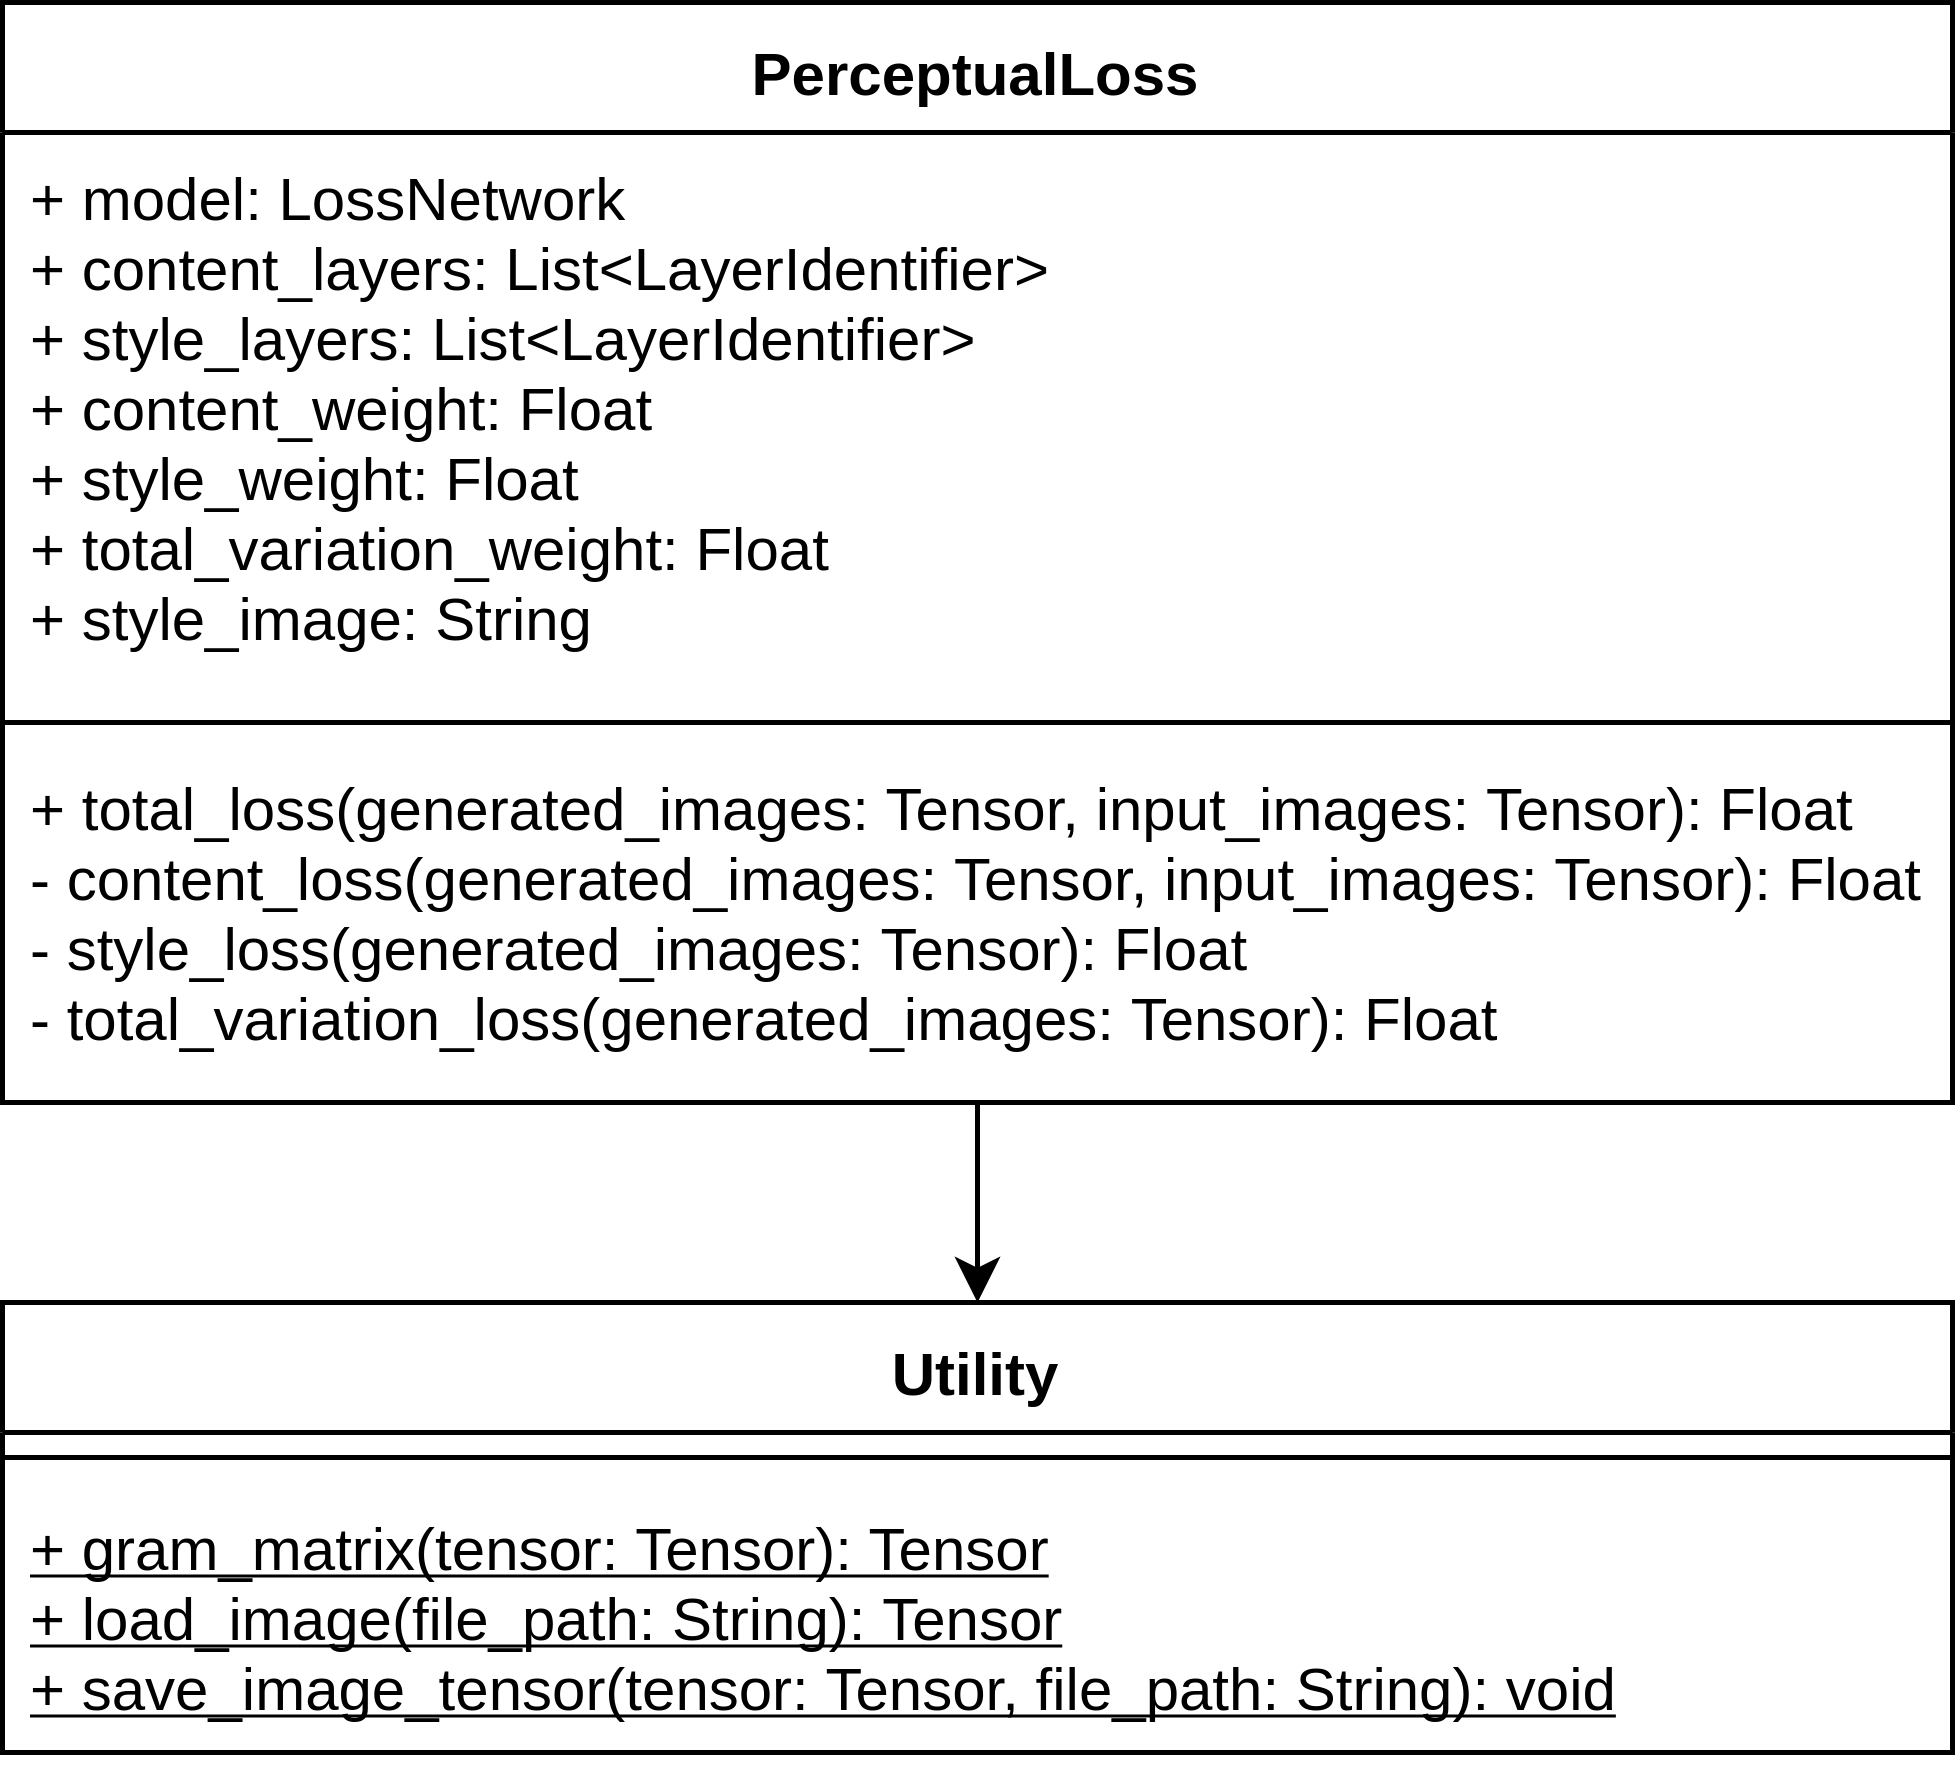
\includegraphics[width=0.50\textwidth]{resources/content/neural_style_class_diagram.png}
	\caption{Komponenten für den Neural Style Algorithmus, eigene Darstellung}
	\label{img:neural_style_class_diagram_img}
\end{figure}

Der Algorithmus wird in einer interaktiven Umgebung erstellt, damit unterschiedliche Kombinationen der Hyperparameter schnell verändert und getestet werden können. Folgender Programmablaufplan skiziert ein entsprechendes Script. Für die Berechnung der mathematisch aufwendigen Aufgaben (z.B. Backprogation \ref{sec:backpropagation}) wird eine ensprechende externe Library, die für solche Aufgaben optimiert wurde, benutzt.

% https://drive.google.com/file/d/1OVpNUtWEs0HbToxkkzMw6EZe5UUVHyme/view?usp=sharing
\begin{figure}[H]
	\centering
	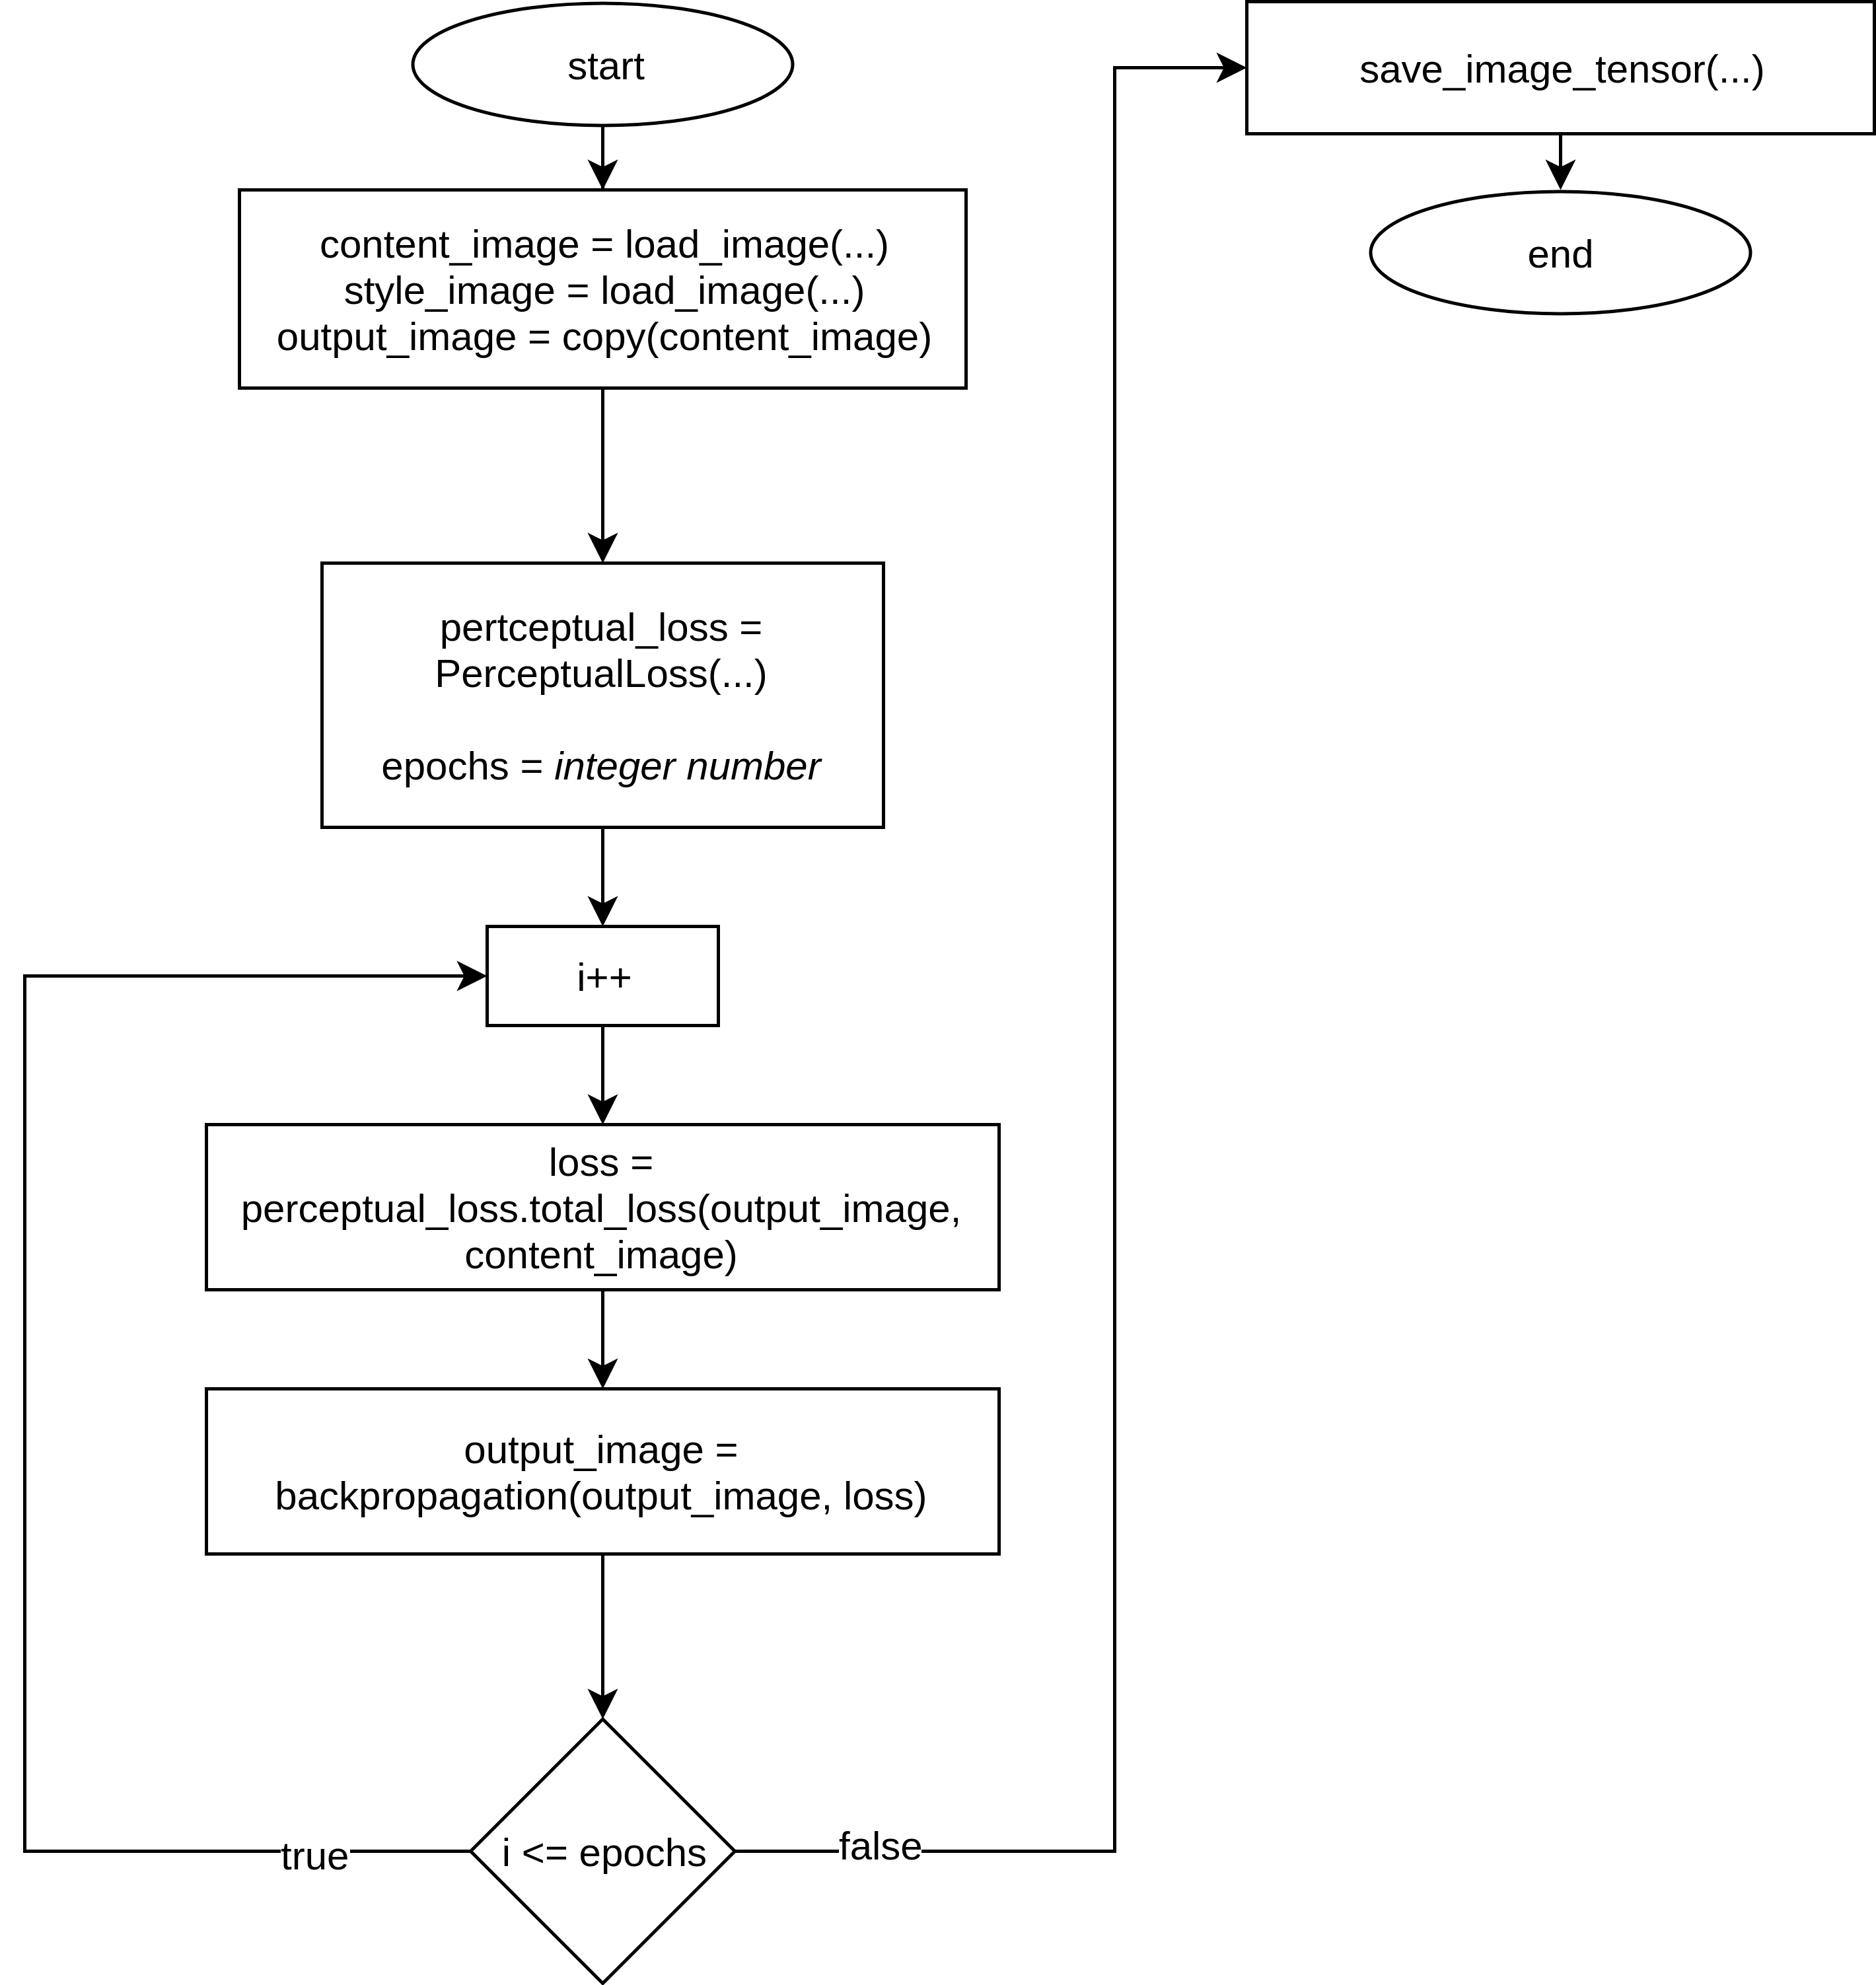
\includegraphics[width=0.75\textwidth]{resources/content/neural_style_pap.png}
	\caption{Programmablaufplan für den Neural Style Algorithmus, eigene Darstellung}
	\label{img:neural_style_pap_img}
\end{figure}

Bei Start des Programms werden das Content-Bild \mintinline{python}{content_image} und das Style-Bild \mintinline{python}{style_image} geladen. Danach wird eine Kopie von \mintinline{python}{content_image} in \mintinline{python}{output_image} erstellt. Die Bilder liegen dann als \gls{tensor}en der Form $ Channel \times Height \times Width $, wobei $ Channel = 3 $ beträgt, da Bilder im RGB-Farbraum drei Farbkanäle aufweisen.

Es wird ein Objekt der Klasse \mintinline{python}{PerceptualLoss} erstellt. Bei der Instanziierung werden die folgenden benötigten Hyperparameter als Argumente dem Konstruktor übergeben:

\begin{itemize}
	\item \mintinline{python}{model}: Das Netzwerk, hier VVG16, dessen \gls{activation_map}s genutzt werden.
	\item \mintinline{python}{content_layers}: Eine Liste von Layern für die Berechnung des Content-Loss.\\ $ \{ relu3\_3 \} $
	\item \mintinline{python}{style_layers}: Eine Liste von Layern für die Berechnung des Style-Loss.\\ $ \{ relu1\_2, relu2\_2, relu3\_3, relu4\_3 \} $
	\item \mintinline{python}{content_weight}: Die Gewichtung des Content-Loss. $ 1 $ 
	\item \mintinline{python}{style_weight}: Die Gewichtung des Style-Loss. $ 1 \times 10^{7} $
	\item \mintinline{python}{total_variation_weight}: Die Gewichtung des Total-Variation-Denoising Faktors. $ 1 \times 10^{-5} $
	\item \mintinline{python}{style_image}: Der \gls{tensor} des gewünschten Style-Bildes.
\end{itemize}

Die Werte orientieren sich an den im Paper \cite{DBLP:journals/corr/JohnsonAL16} verwendeten Hyperparametern. Je nach gewähltem Stil sind jedoch abweichenden Einstellungen erforderlich, um optisch ansprechende Ergebnisse zu erzielen. Auf unterschiedliche Kombinationen der Hyperparameter wird im Kapitel \ref{cha:tests} eingegangen.

\section{Fast Neural Style Transfer}

Die zuvor konzipierte Loss-Funktion kann beim Fast Neural Style Transfer wieder verwendet werden. 
Im Gegensatz zum vorherigen Verfahren werden nicht die Pixel als Parameter anhand der Loss-Funktion optimiert sondern die Gewichtungsparameter eines Neuronalen Netzwerks. Dieses Verfahren wird auch Training genannt. Nach beendeter Trainingsphase ist das Netzwerk in der Lage, willkürliche Bilder in Bilder mit dem mit \mintinline{python}{style_image} ausgewählten Stil umzuwandeln.

Im Zuge dieser Arbeit soll eine Netzwerkarchitektur gefunden werden, die in der Lage ist, diese Aufgabe zu bewältigen. Außerdem wird die Netzwerkarchitektur im Kapitel \ref{cha:tests} auf ihre Performanz auf Geräten mit leistungsarmer Hardware getestet.

\subsection{Aufbau}
\label{sec:aufbau}

Die Netzwerkarchitektur, die beim Fast Neural Style Transfer verwendet wird, nachfolgend Transformer Net genannt, orientiert sich an dem Github-Repository \cite{PyTorchFastNeuralStyle}, dass den Fast Neural Style Transfer implementiert.
Sie besteht aus drei Teilen. Einem Down-Sampling-Teil, einem Computational-Teil (auch Bottleneck genannt) und einem Up-Sampling-Teil.

\begin{figure}[H]
	\centering
	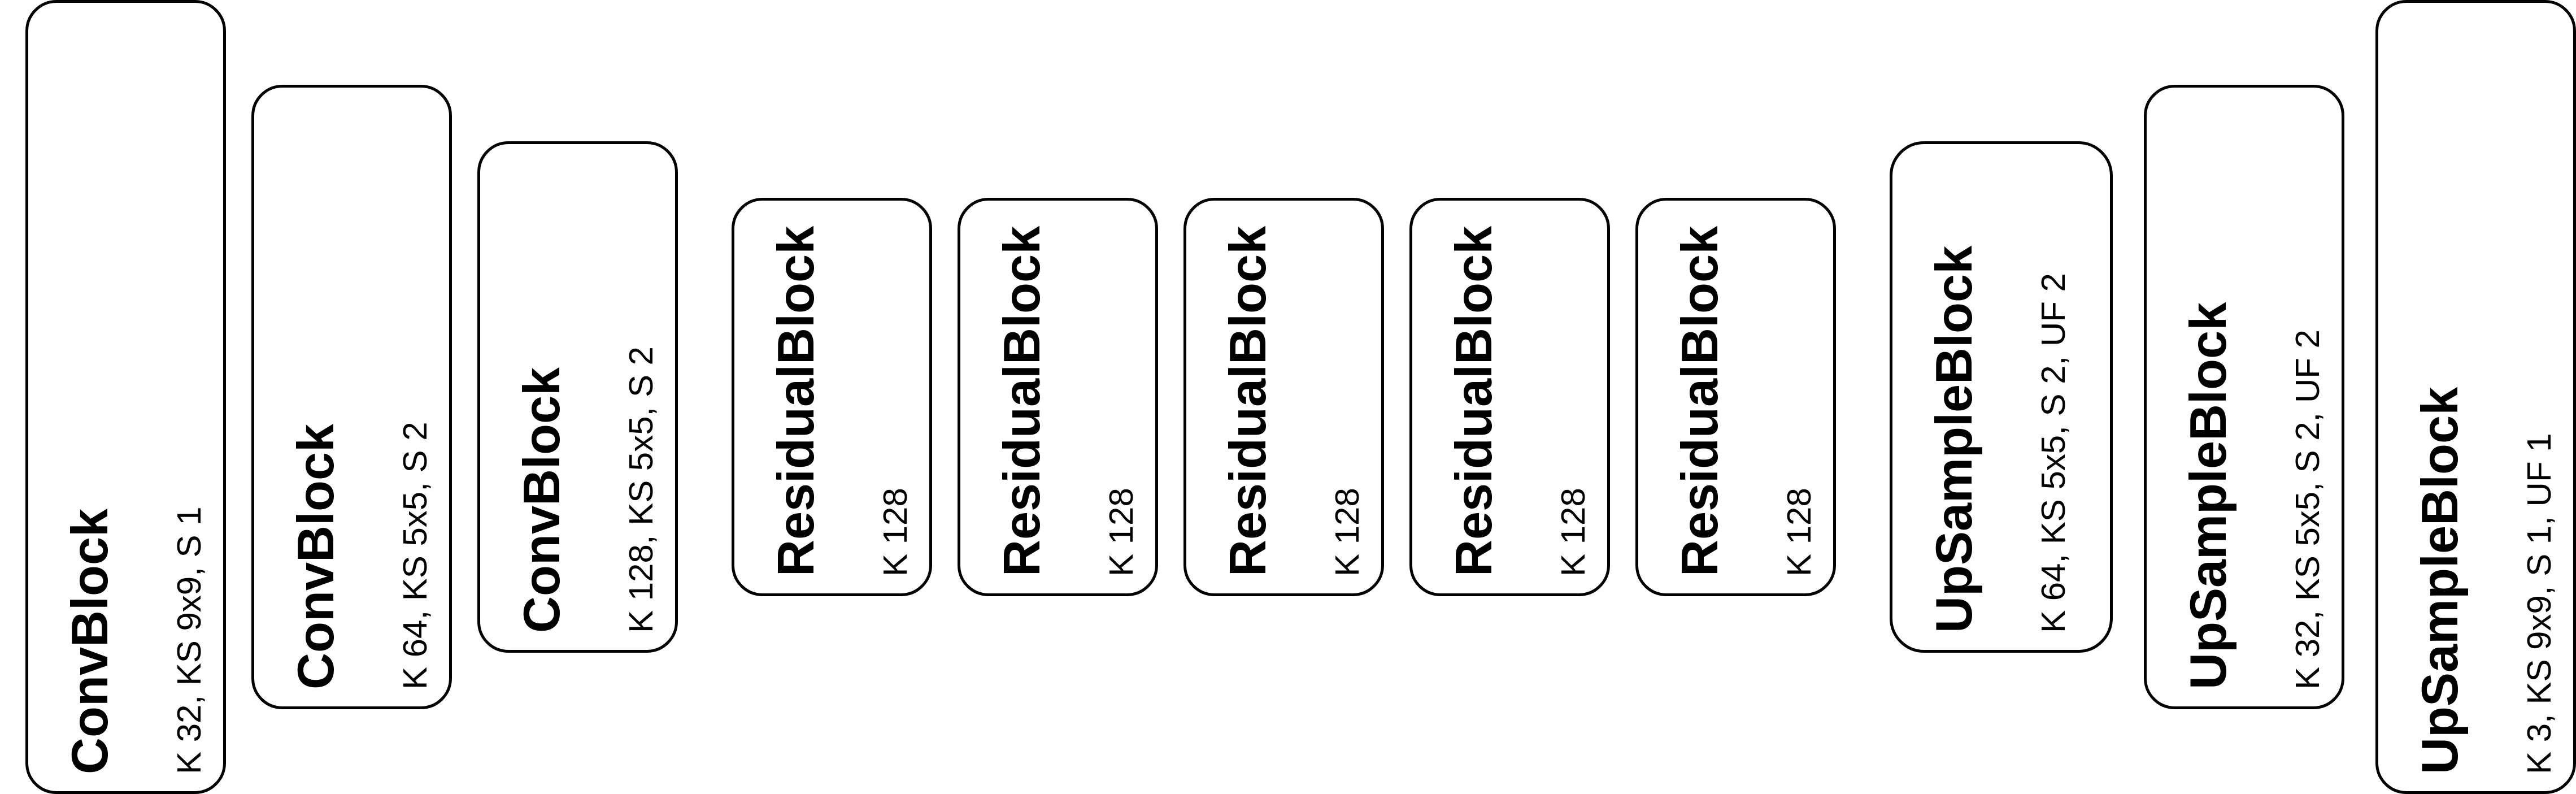
\includegraphics[width=0.90\textwidth]{resources/content/transformer_net.png}
	\caption{Netzwerkarchitektur des Transformer Net, eigene Darstellung}
	\label{img:transformer_net_img}
\end{figure}

Die Abkürzungen in der Grafik stehen für folgende Werte:

\begin{itemize}
	\item K = Anzahl Kernel
	\item KS = Kernel Size
	\item S = Stride
	\item UF = Upsampling Factor
\end{itemize}

Im ersten Teil, bestehend aus Convolutional Blöcken, wird durch die Verwendung des Stride Paramters das Eingangsbild hinter jedem Layer verkleinert.
Mit einem Stride von zwei, wird das Bild ungefähr um die Hälfte der ursprünglichen Größe verkleinert, vgl Kapitel \ref{cha:fundamentals}. Dabei wird die Anzahl der Channels mit jedem Block vergrößert um den Informationsverlust, der durch die verkleinerten Bilder entsteht, auszugleichen.

\begin{figure}[H]
	\centering
	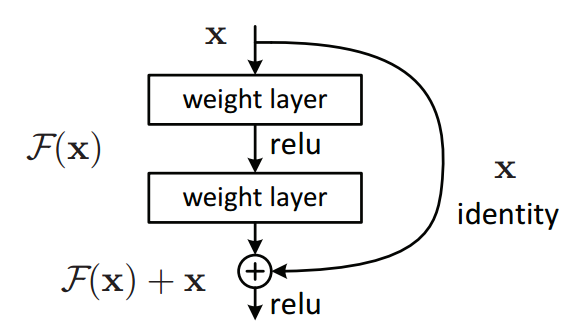
\includegraphics[width=0.50\textwidth]{resources/content/residual_block.png}
	\caption{Aufbau eines Residual Block \cite{residual_block_img}}
	\label{img:residual_block_img}
\end{figure}

Der zweite Teil besteht aus Residual Blöcken, beschrieben in \cite{DBLP:journals/corr/HeZRS15}. Diese bestehen aus zwei aufeinanderfolgenden Convolutional Layern, die mit einer sogennanten Skip-Connection mit ihren Eingangsdaten verbunden sind. Das hat den Vorteil, dass die ursprünglichen Eingangsdaten nach jedem Layer noch vorhanden sind. Das beugt dem \gls{vanishing_gradient} Problem vor. In diesem Teil des Netzwerk entsteht die meiste Berechnung und die meisten Daten des Stils werden hier in den Gewichten der Kernels gespeichert.

Im dritten Teil wird das Bild durch Upsampling wieder auf seine ursprüngliche Maße vergrößert. Außerdem werden die Channels auf drei reduziert um es als RGB-Bild anzeigen zu können. Die Vergrößerung wird durch Nearest Neighbor Interplolation kombiniert mit einem Convolutional Layer realisiert.
Es wird zusammen mit seinen Vorteilen in \cite{odena2016deconvolution} näher beschrieben.

\pagebreak

\subsection{Unterschiedliche Netzwerkgrößen}

Wie auf der Grafik \ref{img:transformer_net_img} zu erkennen ergibt sich die Anzahl der Channels jeweils aus dem einem Potenzwert der Basis $ 2 $ multipliziert mit eine Multiplikator $ m $, in diesem Fall der Wert $ 32 $.

\begin{align}
	& c_{1}(m) = m * 2^{0}
	& 32 = 32 * x^{0}
\end{align}

\begin{align}
	& c_{2}(m) = m * 2^{1}
	& 64 = 32 * x^{1}
\end{align}

\begin{align}
	& c_{3}(m) = m * 2^{2}
	& 128 = 32 * x^{2}
\end{align}

Durch den Multiplikator $ m $ lässt sich Netzwerkgröße und somit die Anzahl der Parameter einstellen. Unterschiedliche Netzwerkgrößen sind der Lage die Stile unterschiedlich gut festzuhalten. Auch wirkt sich die Netzwerkgröße auf die Berechnungs- und Trainingszeit des Netzwerks aus, was unter dem Gesichtspunkt der Verwedung auf Geräten mit leistungsarmer Hardware eine Rolle spielt.

Neben dem Multiplikator gibt es einen weiteren Parameter der die Netzwerkgröße verändert. Der Anzahl der ResidualBlocks im Computational-Teil als $ s $ bezeichnet. Im Kapitel \ref{cha:tests} werden unterschiedliche Netzwerkgrößen und ihre Performanz getestet.